
\item The figure below shows the variation of specific heat capacity (\(C\)) of a solid as a function of temperature (\(T\)). The temperature is increased continuously from 0 to 500 K at a constant rate. Ignoring any volume change, the following statement(s) is (are) correct to a reasonable approximation.
    \begin{center}
        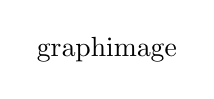
\begin{tikzpicture}
            \node at (0, 0) {graphimage}; % Replace 'graph_image' with actual filename
        \end{tikzpicture}
    \end{center}
    \begin{tasks}(1)
        \task the rate at which heat is absorbed in the range 0-100 K varies linearly with temperature \(T\).
        \task heat absorbed in increasing the temperature from 0-100 K is less than the heat required for increasing the temperature from 400-500 K.
        \task there is no change in the rate of heat absorption in the range 400-500 K.
        \task the rate of heat absorption increases in the range 200-300 K.
    \end{tasks}
